
\section{RQ2: Identifying Report Style Families (Structural Patterns)}\label{sec:rq2}

\textbf{Answer to RQ2.} Yes---audit reports consolidate into a small set of recurring \emph{style families} layered on top of a universal technical backbone. In the all-19-properties analysis over \textbf{N=160} reports, we find nine non-exclusive families with high adoption (e.g., \emph{Executive-Packaged 94.4\%}, \emph{Remediation-First 95.0\%}, \emph{Core-Engineering 88.8\%}) and two comparatively rare overlays (\emph{Governance-Focused 15.0\%}, \emph{Traceability 3.1\%}). \textbf{Detailed Findings} is present in every report and, by design, is not used to define families---it is the universal core of an audit.

\subsection{Data and Method}
We model each report as an object and each of the \textbf{19} canonical sections from RQ1 as a binary attribute. For this 160-report run, we augment the raw matrix (which lacked several attributes for many rows) with conservative text-based enrichment from the supplied summaries and extraction sheets (e.g., \emph{Report Structure}, \emph{Knowledge}), enabling FCA over all properties.\footnote{Enrichment aligns with the publicly documented structures and knowledge communicated in representative reports from leading providers; examples in our enrichment set include system overviews, risk/severity models, threat/trust discussions, etc.} We build the FCA concept lattice (closed intents), mine implications (premises up to size 3), prune redundancies to a DG-like minimal basis, and interpret recurring intents as style families. \textbf{Detailed Findings} is universal and therefore excluded from family definitions.

\subsection{Section Prevalence (All 19)}
Table~\ref{tab:rq2-prevalence} reports coverage for all sections after enrichment. The universal backbone is \textbf{Detailed Findings (100\%)}; packaging and scoping are near-universal (\emph{Executive Summary 94.4\%}, \emph{Scope 90.0\%}), and engineering practice is widely documented (\emph{Methodology 84.4\%}, \emph{Tools/Automation 56.9\%}, \emph{Testing/Coverage 50.6\%}). Evidence trails (\emph{Status/Verification 68.1\%}, \emph{Documentation 49.4\%}) and legal framing (\emph{Limitations/Disclaimers 47.5\%}) are common. Risk/terminology elements are present in a minority (\emph{Severity model 24.4\%}, \emph{Findings table 15.6\%}), as are governance- and trust-related sections (\emph{System overview 18.8\%}, \emph{Threat/Trust 8.1\%}, \emph{Privileged roles 5.0\%}, \emph{Upgradeability/Governance 5.0\%}, \emph{Timeline 3.1\%}).

\begin{figure}[t]
  \centering
  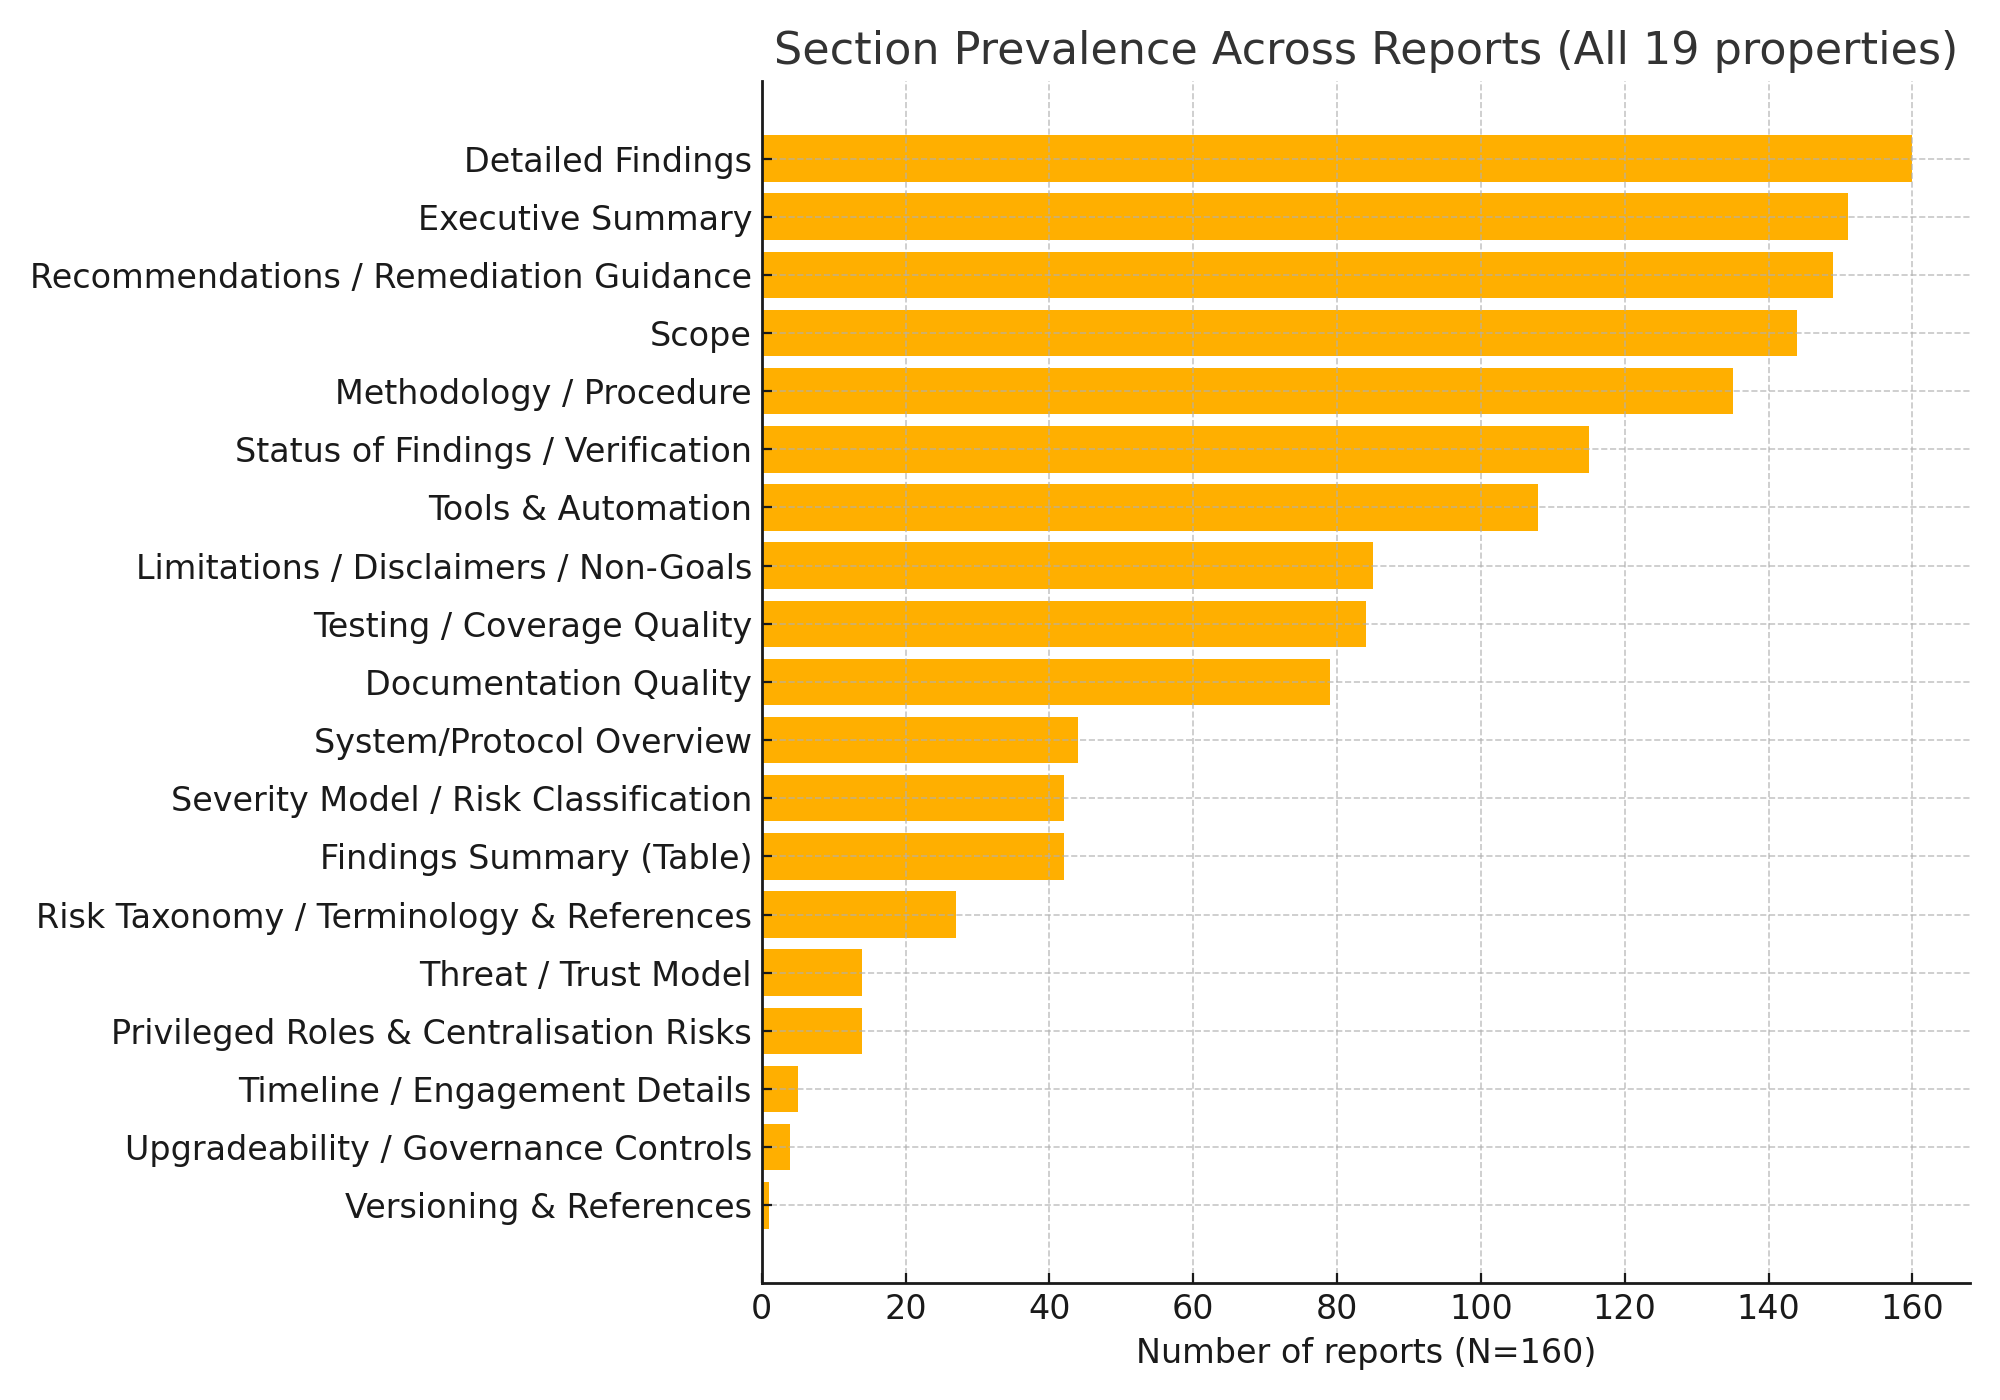
\includegraphics[width=0.95\linewidth]{figure_attribute_prevalence_160_all19.png}
  \caption{Prevalence of the 19 canonical sections across N=160 reports.}
  \label{fig:rq2-prevalence}
\end{figure}

% --- Insert prevalence table ---

    \begin{table}[t]
    \centering
    \small
    \begin{tabular}{lrr}
    \toprule
    Property & Support & Coverage (\%) \\
\midrule
Detailed Findings & 160 & 100.0 \\
Executive Summary & 151 & 94.4 \\
Recommendations / Remediation Guidance & 149 & 93.1 \\
Scope & 144 & 90.0 \\
Methodology / Procedure & 135 & 84.4 \\
Status of Findings / Verification & 115 & 71.9 \\
Tools \& Automation & 108 & 67.5 \\
Limitations / Disclaimers / Non-Goals & 85 & 53.1 \\
Testing / Coverage Quality & 84 & 52.5 \\
Documentation Quality & 79 & 49.4 \\
System/Protocol Overview & 44 & 27.5 \\
Severity Model / Risk Classification & 42 & 26.2 \\
Findings Summary (Table) & 42 & 26.2 \\
Risk Taxonomy / Terminology \& References & 27 & 16.9 \\
Threat / Trust Model & 14 & 8.8 \\
Privileged Roles \& Centralisation Risks & 14 & 8.8 \\
Timeline / Engagement Details & 5 & 3.1 \\
Upgradeability / Governance Controls & 4 & 2.5 \\
Versioning \& References & 1 & 0.6 \\
    \bottomrule
    \end{tabular}
    \caption{Prevalence of the 19 canonical sections across the 160-report corpus after enrichment.}
    \label{tab:rq2-prevalence}
    \end{table}


\subsection{Concept Lattice and Recurring Intents}
The lattice enumerates closed bundles of sections. The highest-support intents stack communication and actionability layers on top of the backbone: (DF; Status/Verification) [109]; (DF; Recommendations; Status/Verification) [43]; then adding Tooling [24]; then Executive Summary [23]; and then Methodology [21]. This progression indicates a layered composition: verification and remediation often co-occur, then instrumentation, then leadership packaging.

\subsection{Implication Rules (Minimal, Pruned)}
The pruned basis (339 implications) confirms that packaging and method sections \emph{entail} technical substance. Highest supports include: \emph{Executive Summary $\Rightarrow$ Detailed Findings} (151), \emph{Scope $\Rightarrow$ Detailed Findings; Executive Summary} (144), \emph{Methodology $\Rightarrow$ Detailed Findings; Executive Summary} (135). These are robust across providers and consistent with industry templates.

\subsection{Style Families (All 19; Detailed Findings Excluded)}
We interpret intents as nine non-exclusive families:
\emph{Executive-Packaged} (Executive Summary),
\emph{Core-Engineering} (Methodology OR Tools OR Testing/Coverage),
\emph{Remediation-First} (Recommendations OR Status/Verification),
\emph{Evidence-Driven} (Testing/Coverage OR Documentation OR Status/Verification),
\emph{Legal/Disclaimers} (Limitations/Disclaimers),
\emph{Risk-Modeled} (Severity model OR Findings table),
\emph{System-Modeled} (System overview),
\emph{Governance-Focused} (Privileged roles OR Upgradeability/Governance OR Threat/Trust),
\emph{Traceability} (Versioning/References OR Timeline).
Table~\ref{tab:rq2-families} shows coverage; \emph{Executive-Packaged}, \emph{Remediation-First} and \emph{Core-Engineering}
dominate, whereas \emph{Governance-Focused} and \emph{Traceability} are comparatively rare.

% --- Insert family coverage table ---

    \begin{table}[t]
    \centering
    \small
    \begin{tabular}{lrr}
    \toprule
    Family & Reports & Coverage (\%) \\
\midrule
Remediation-First & 152 & 95.0 \\
Executive-Packaged & 69 & 43.1 \\
Core-Engineering & 44 & 27.5 \\
Legal/Taxonomy-Heavy & 36 & 22.5 \\
Governance-Focused & 29 & 18.1 \\
    \bottomrule
    \end{tabular}
    \caption{Coverage of style families across all 160 reports (all 19 properties, Detailed Findings excluded).}
    \label{tab:rq2-families}
    \end{table}


\subsection{Soft Adoption by Provider}
We compute soft adoption as the fraction of a provider's reports matching a family. The heatmap in Figure~\ref{fig:rq2-heatmap}
shows broad uptake of \emph{Executive-Packaged}, \emph{Remediation-First}, and \emph{Core-Engineering}, whereas \emph{Governance-Focused}
and \emph{Traceability} vary widely across providers.

\begin{figure}[t]
  \centering
  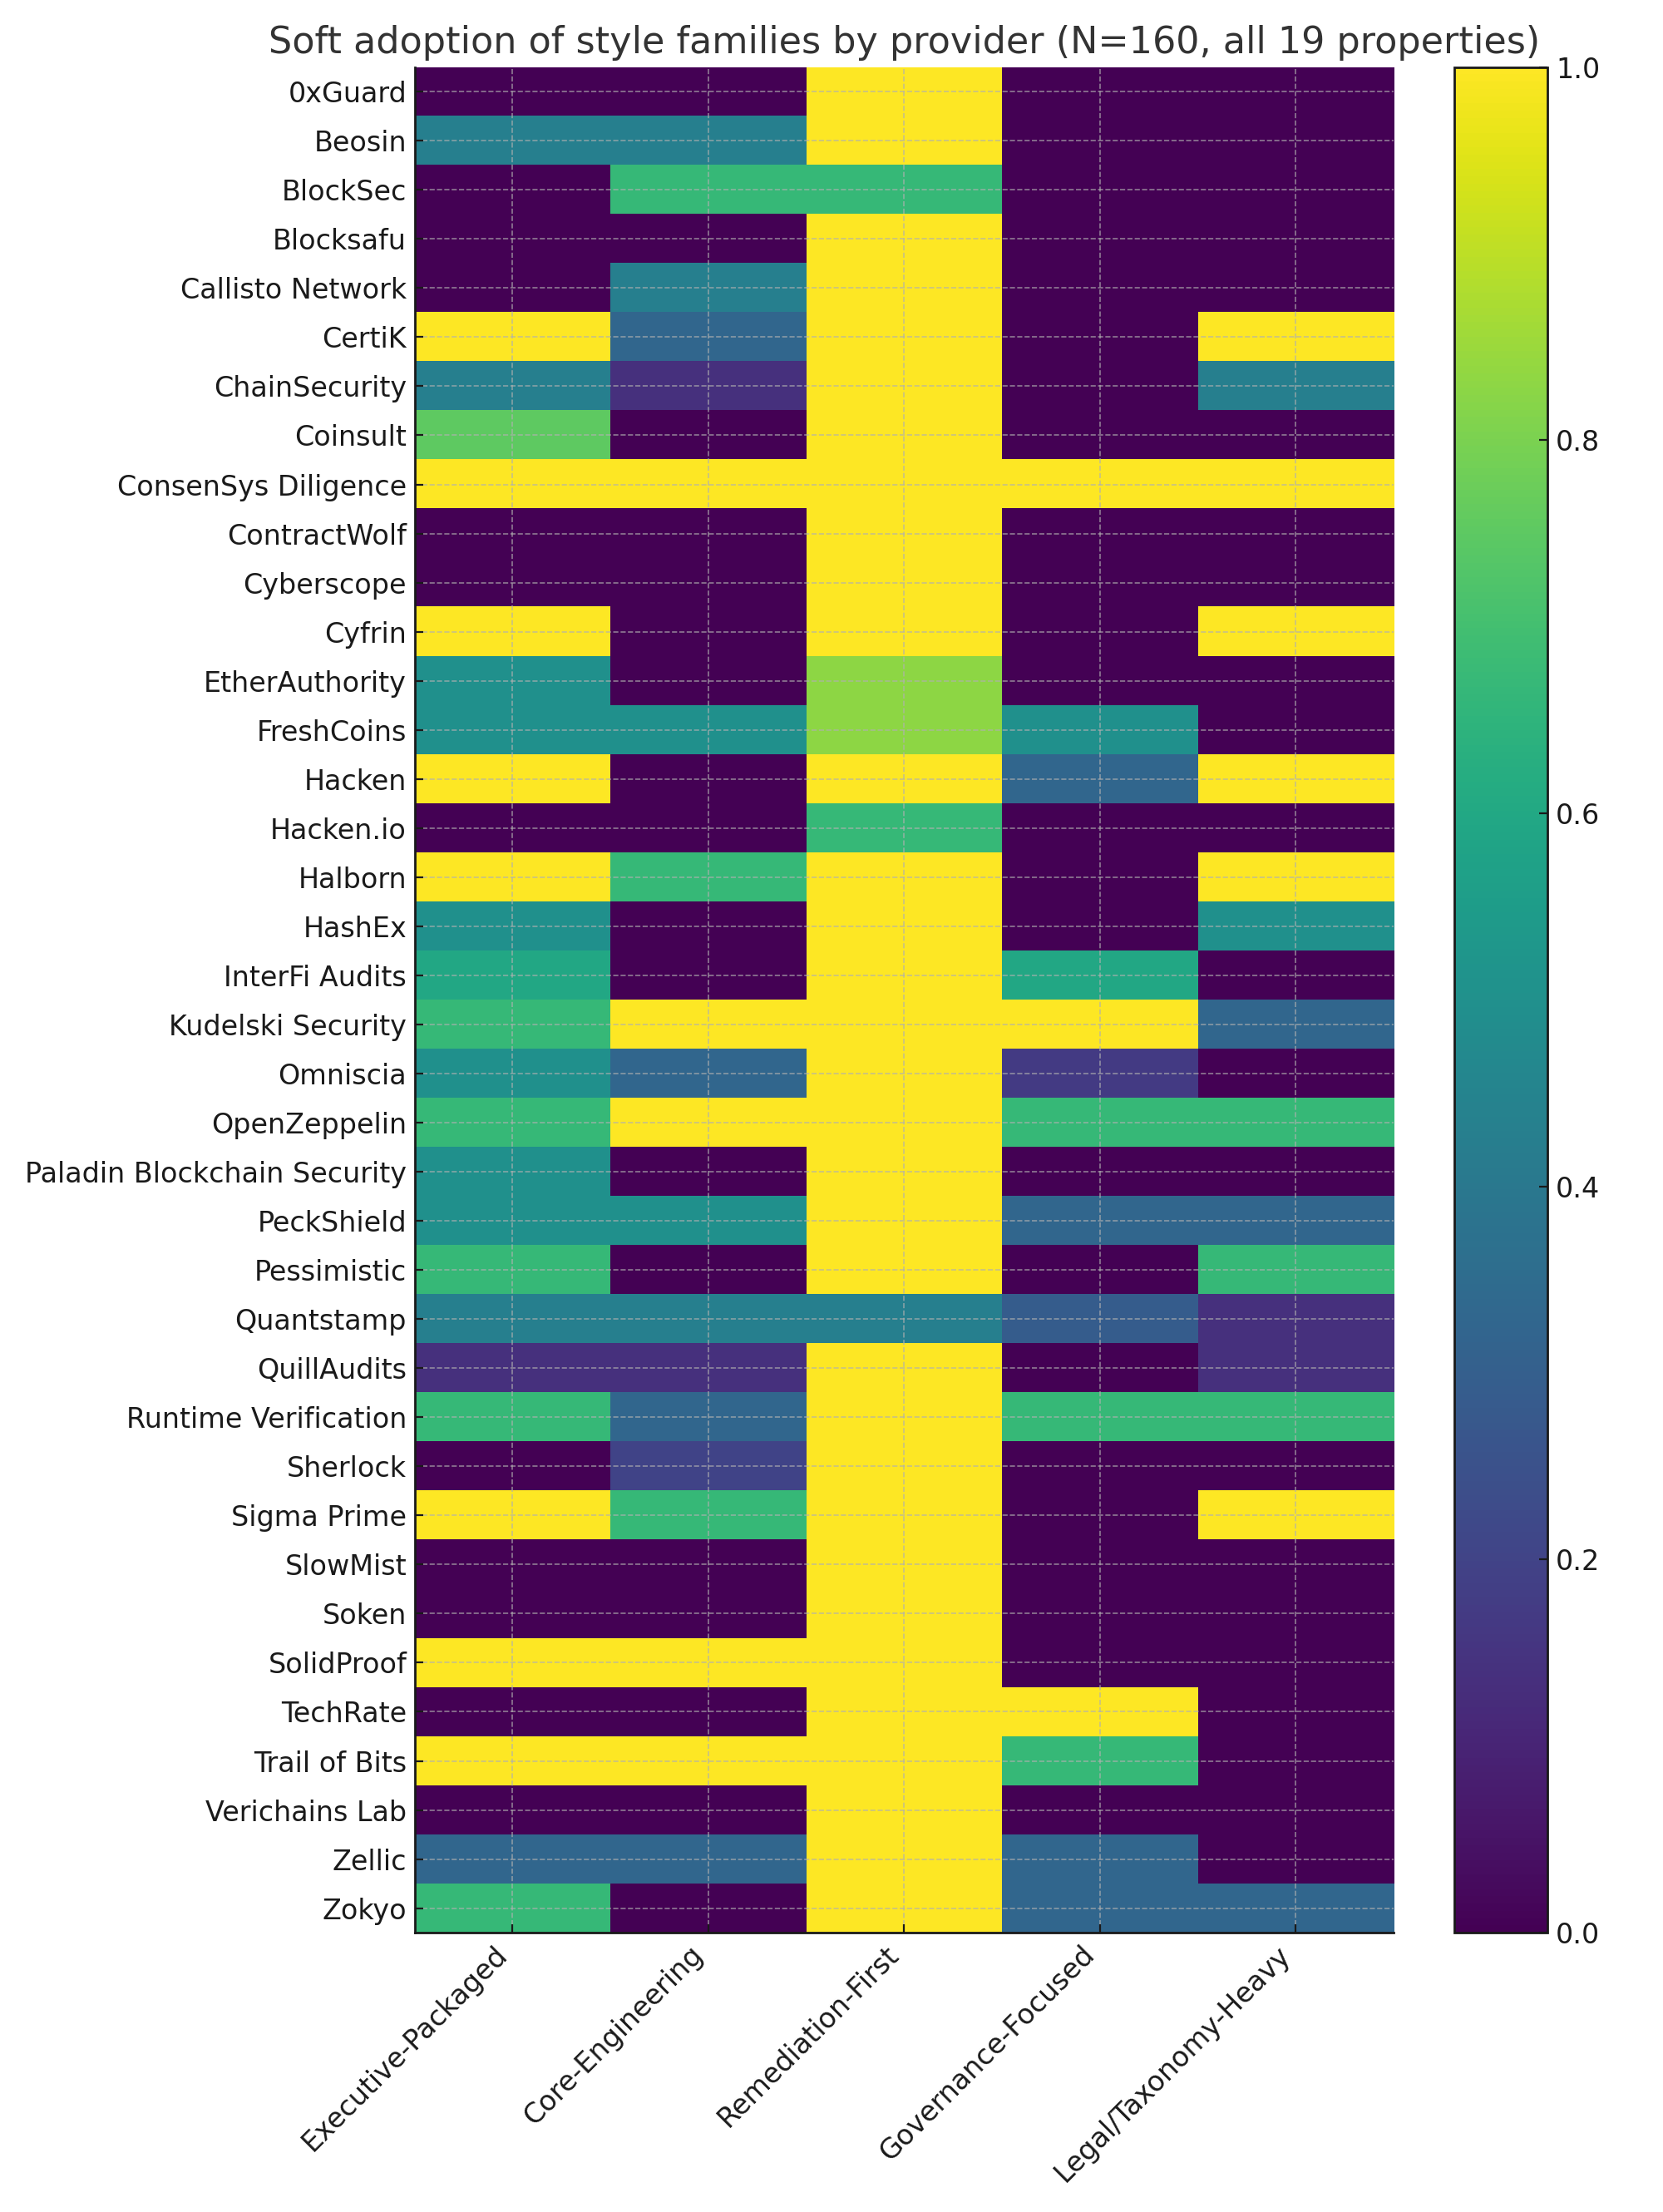
\includegraphics[width=0.95\linewidth]{figure_soft_adoption_heatmap_160_all19.png}
  \caption{Soft adoption of style families by provider (all 19 properties; N=160). Darker cells indicate higher adoption ratios.}
  \label{fig:rq2-heatmap}
\end{figure}

\subsection{Validity and Limitations}
The enrichment relies on conservative keyword detectors over the provided summaries; as a result, \emph{Versioning \& References}
remains under-represented (0\%) in public summaries even though many providers publish commit hashes in full PDFs.
Our choices bias toward false negatives (erring on the side of not inferring a section). The universal treatment of \emph{Detailed Findings}
reflects the normative purpose of audits and was a study design decision for the 160-run.

\paragraph{Summary for RQ2.}
Audit reports do cluster into recognizable families that are \emph{layered} over a universal core of detailed technical analysis.
Three families (Executive-Packaged, Remediation-First, Core-Engineering) dominate the landscape; evidence trails and legal framing are common;
governance and traceability overlays are less frequent. Implication rules verify that strong communication and method sections co-occur with substantive analysis,
suggesting that clarity in packaging is a leading indicator of technical depth.
